
\documentclass[10pt]{article}
\usepackage[utf8]{inputenc}
\usepackage{graphicx}
\usepackage{amsmath, amssymb}
\usepackage{geometry}
\usepackage{caption} 
\geometry{a4paper, margin=0.5in, landscape} 

\begin{document}

\section*{Comparative EIS Kinetics Report}
\textbf{Model Structure:} \texttt{R0-p(R1-p(R2-Wo2,CPE2),CPE1)}

\begin{center}
    \includegraphics[width=0.45\textwidth]{circuit_2RC_Wo.png}
\end{center}

\renewcommand{\arraystretch}{1.6} 
\begin{table}[h!]
    \centering
    \footnotesize
    \begin{tabular}{|l|c|c|c|c|c|c|}
        \hline
        \textbf{Element} & \textbf{Unit} & \textbf{Bounds} & \textbf{Cauvel\_1\_Lcystine\_24H} & \textbf{Cauvel\_1\_Lcystine\_48H} & \textbf{Cauvel\_1\_Lcystine\_72H} & \textbf{Cauvel\_1\_Lcystine\_168H} \\ \hline
        $R_{0}$ & $\Omega$ & $[1.0e-03, 1.0e+03]$ & $7.77e+01 \pm 3.5e-01$ & $8.03e+01 \pm 3.5e-01$ & $7.91e+01 \pm 2.6e-01$ & $8.31e+01 \pm 5.6e-01$ \\ \hline
        $R_{1}$ & $\Omega$ & $[1.0e+00, 1.0e+08]$ & $3.15e+05 \pm 9.6e+04$ & $2.27e+05 \pm 5.2e+03$ & $3.07e+05 \pm 3.8e+03$ & $3.82e+05 \pm 2.1e+05$ \\ \hline
        $R_{2}$ & $\Omega$ & $[1.0e+00, 1.0e+08]$ & $2.85e+00 \pm 1.1e+05$ & $1.55e+04 \pm 5.2e+03$ & $1.37e+06 \pm 1.4e+00$ & $1.63e+03 \pm 2.1e+05$ \\ \hline
        $W_{2,R}$ & $\Omega$ & $[1.0e-05, 1.0e+07]$ & $2.59e+03 \pm 4.0e+05$ & $2.86e-01 \pm 2.1e+04$ & $1.41e+01 \pm 9.2e-01$ & $6.83e-03 \pm 1.7e+03$ \\ \hline
        $W_{2,\tau}$ & sec & $[1.0e-06, 1.0e+04]$ & $6.27e-01 \pm 9.8e+01$ & $1.15e-04 \pm 8.4e+00$ & $8.55e+01 \pm 6.2e-02$ & $3.03e+00 \pm 2.2e+03$ \\ \hline
        $Q_{2}$ & $\Omega$$^{-1}$ sec$^{a}$ & $[1.0e-11, 1.0e-03]$ & $1.05e-11 \pm 6.4e-04$ & $1.02e-11 \pm 1.6e-05$ & $2.49e-04 \pm 4.2e-05$ & $1.64e-04 \pm 3.3e-02$ \\ \hline
        $n_{2}$ & - & $[5.0e-01, 1.0e+00]$ & $9.68e-01 \pm 8.4e+05$ & $1.00e+00 \pm 1.8e+05$ & $1.00e+00 \pm 6.1e-02$ & $9.99e-01 \pm 3.4e+01$ \\ \hline
        $Q_{1}$ & $\Omega$$^{-1}$ sec$^{a}$ & $[1.0e-11, 1.0e-03]$ & $9.97e-06 \pm 1.3e-07$ & $1.01e-05 \pm 7.5e-08$ & $9.85e-06 \pm 4.0e-08$ & $9.82e-06 \pm 1.9e-07$ \\ \hline
        $n_{1}$ & - & $[5.0e-01, 1.0e+00]$ & $8.62e-01 \pm 2.2e-03$ & $8.50e-01 \pm 3.4e-03$ & $8.44e-01 \pm 8.3e-04$ & $8.33e-01 \pm 3.2e-03$ \\ \hline
        \textbf{$\chi^2$} & - & -  & $3.821e-04$ & $2.634e-04$ & $1.990e-04$ & $7.712e-04$ \\ \hline

    \end{tabular}
\end{table}


\newpage
\section*{Analysis Results: 24H}
\begin{center}
    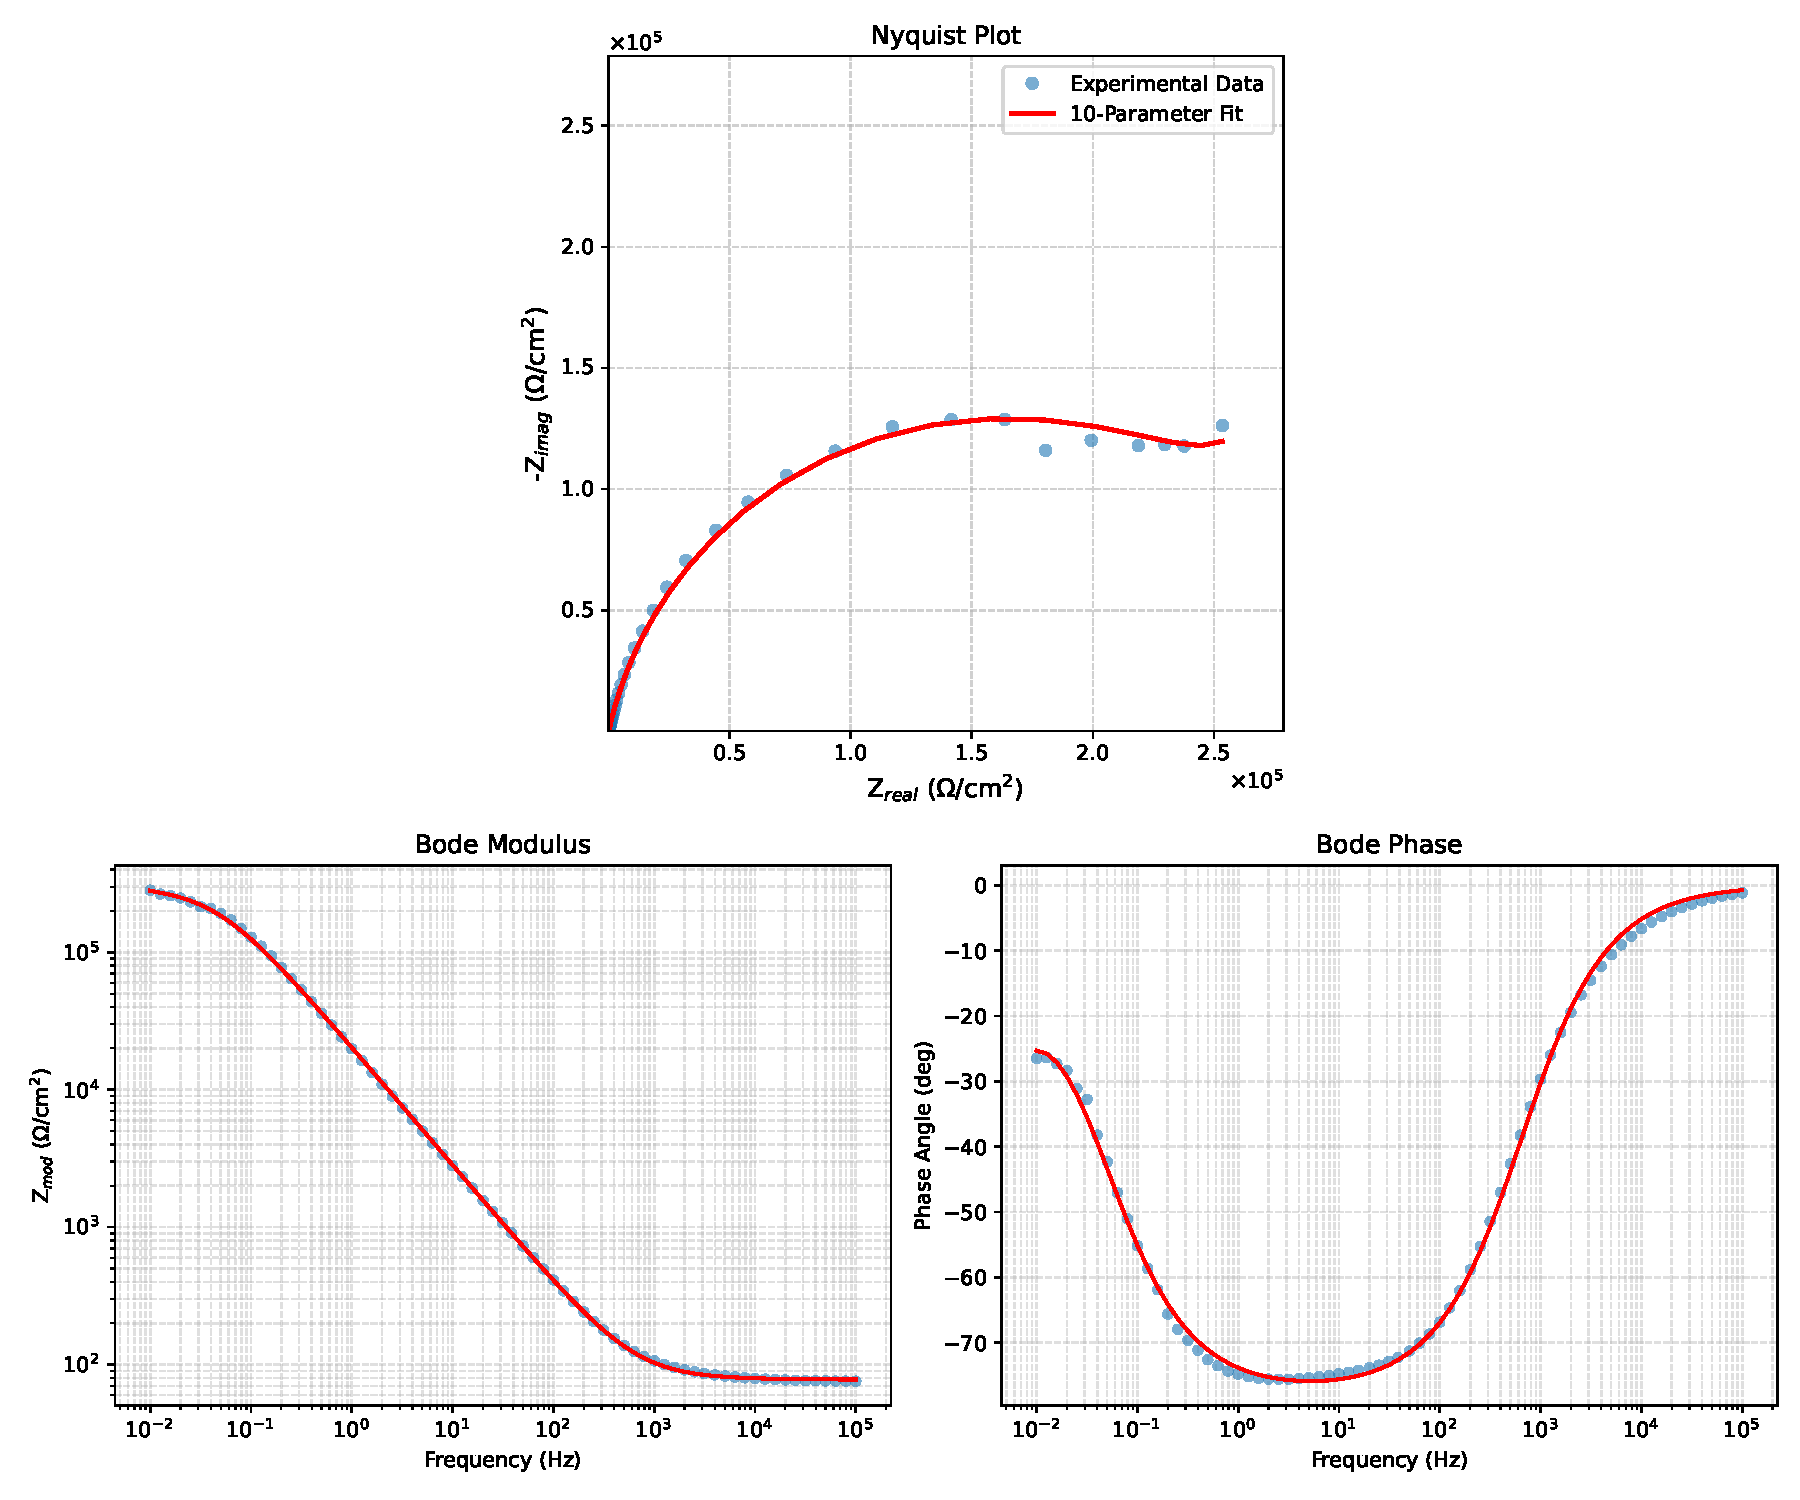
\includegraphics[width=0.7\textwidth]{plots_Cauvel_1_Lcystine_24H.pdf}
    \captionof{figure}{EIS Fit Results for Cauvel\_1\_Lcystine\_24H}
\end{center}

\newpage
\section*{Analysis Results: 48H}
\begin{center}
    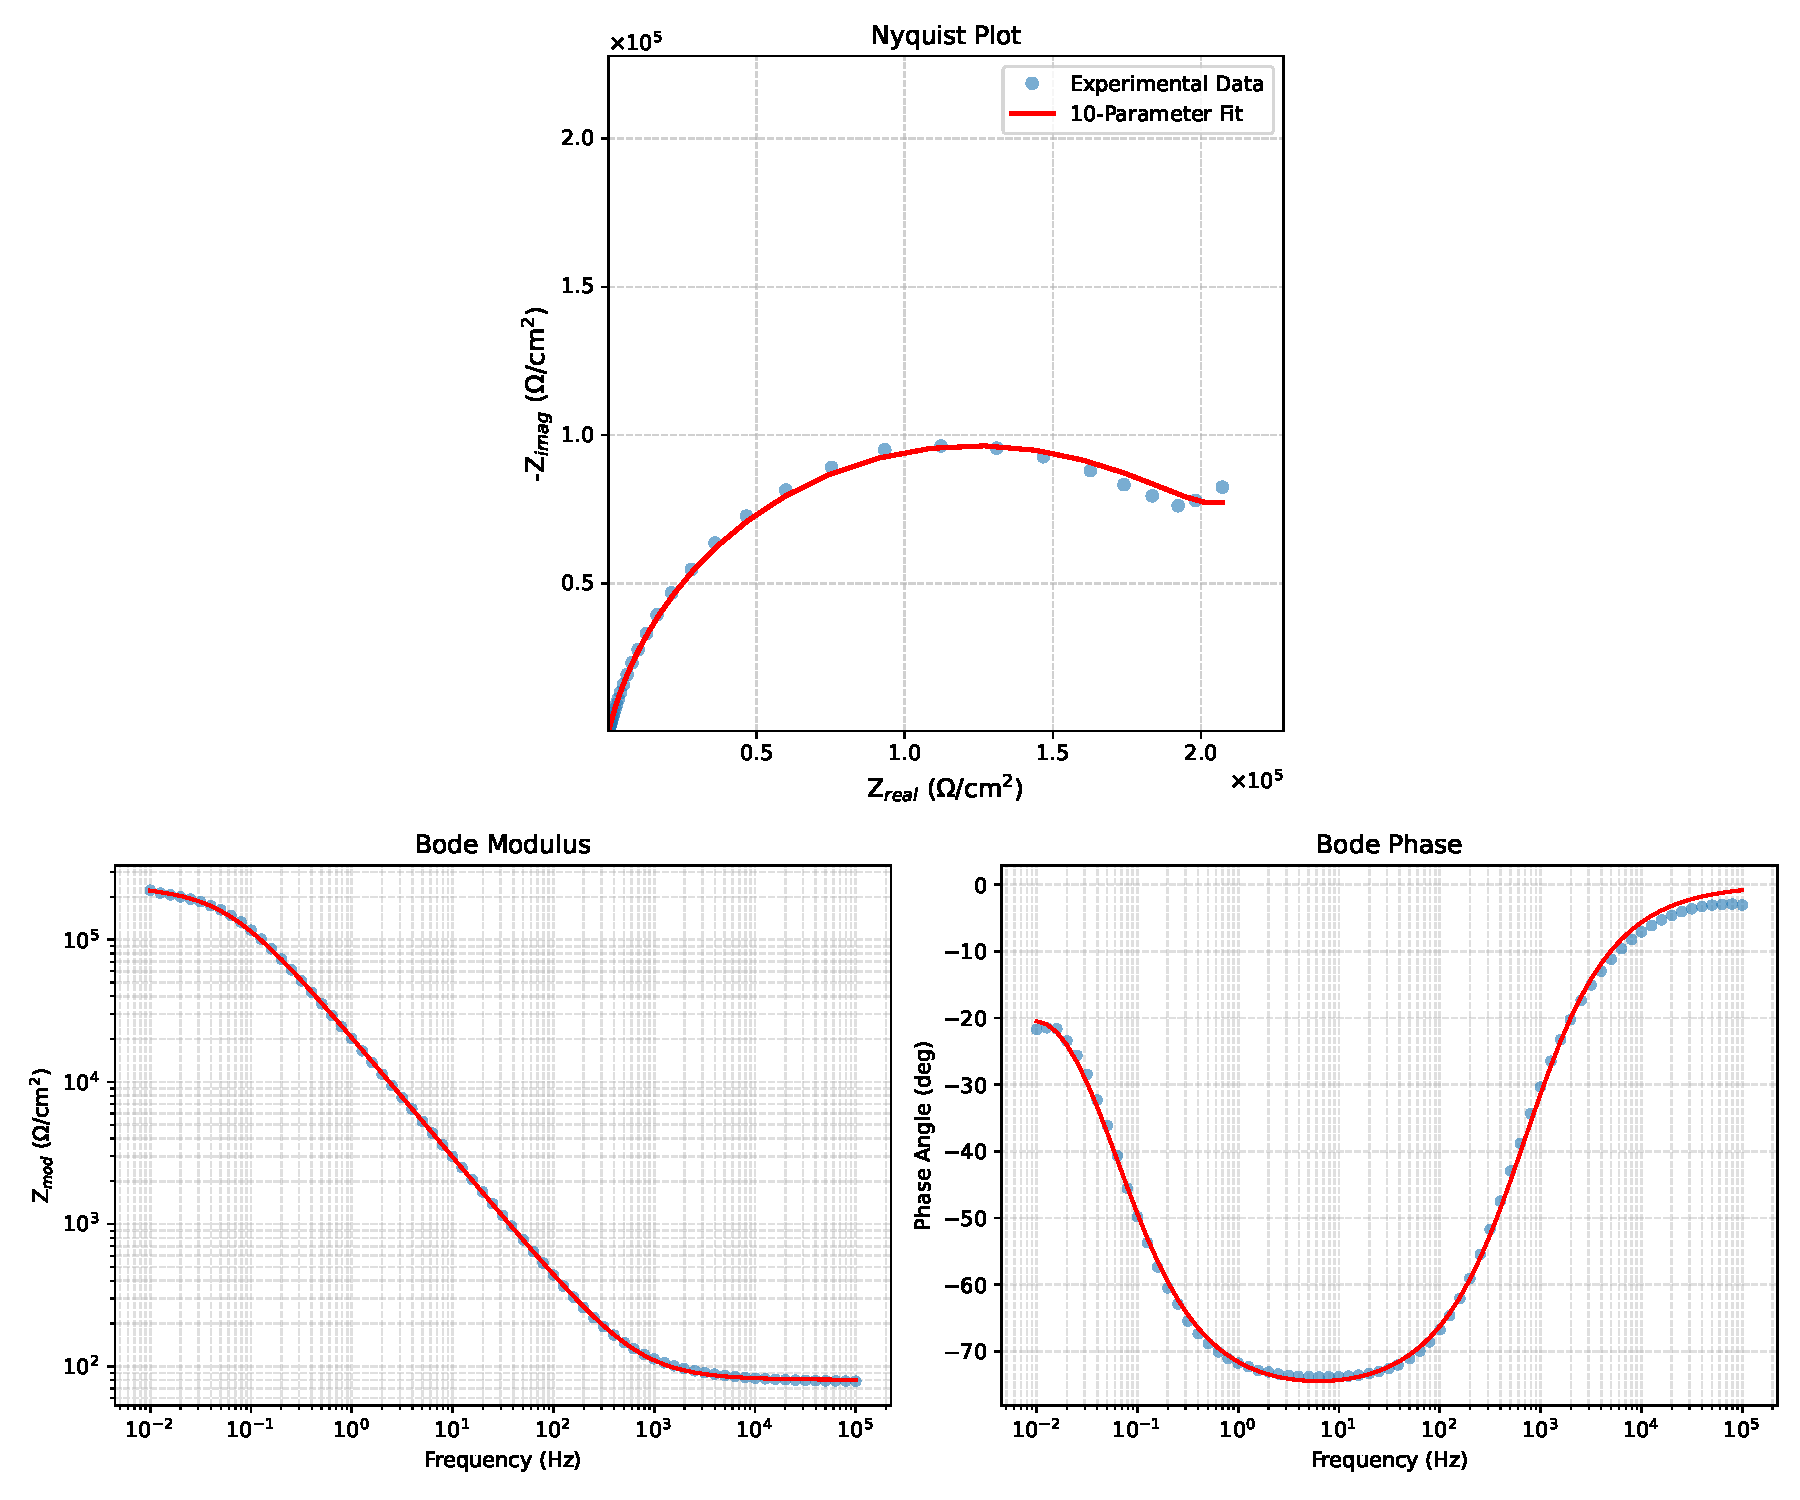
\includegraphics[width=0.7\textwidth]{plots_Cauvel_1_Lcystine_48H.pdf}
    \captionof{figure}{EIS Fit Results for Cauvel\_1\_Lcystine\_48H}
\end{center}

\newpage
\section*{Analysis Results: 72H}
\begin{center}
    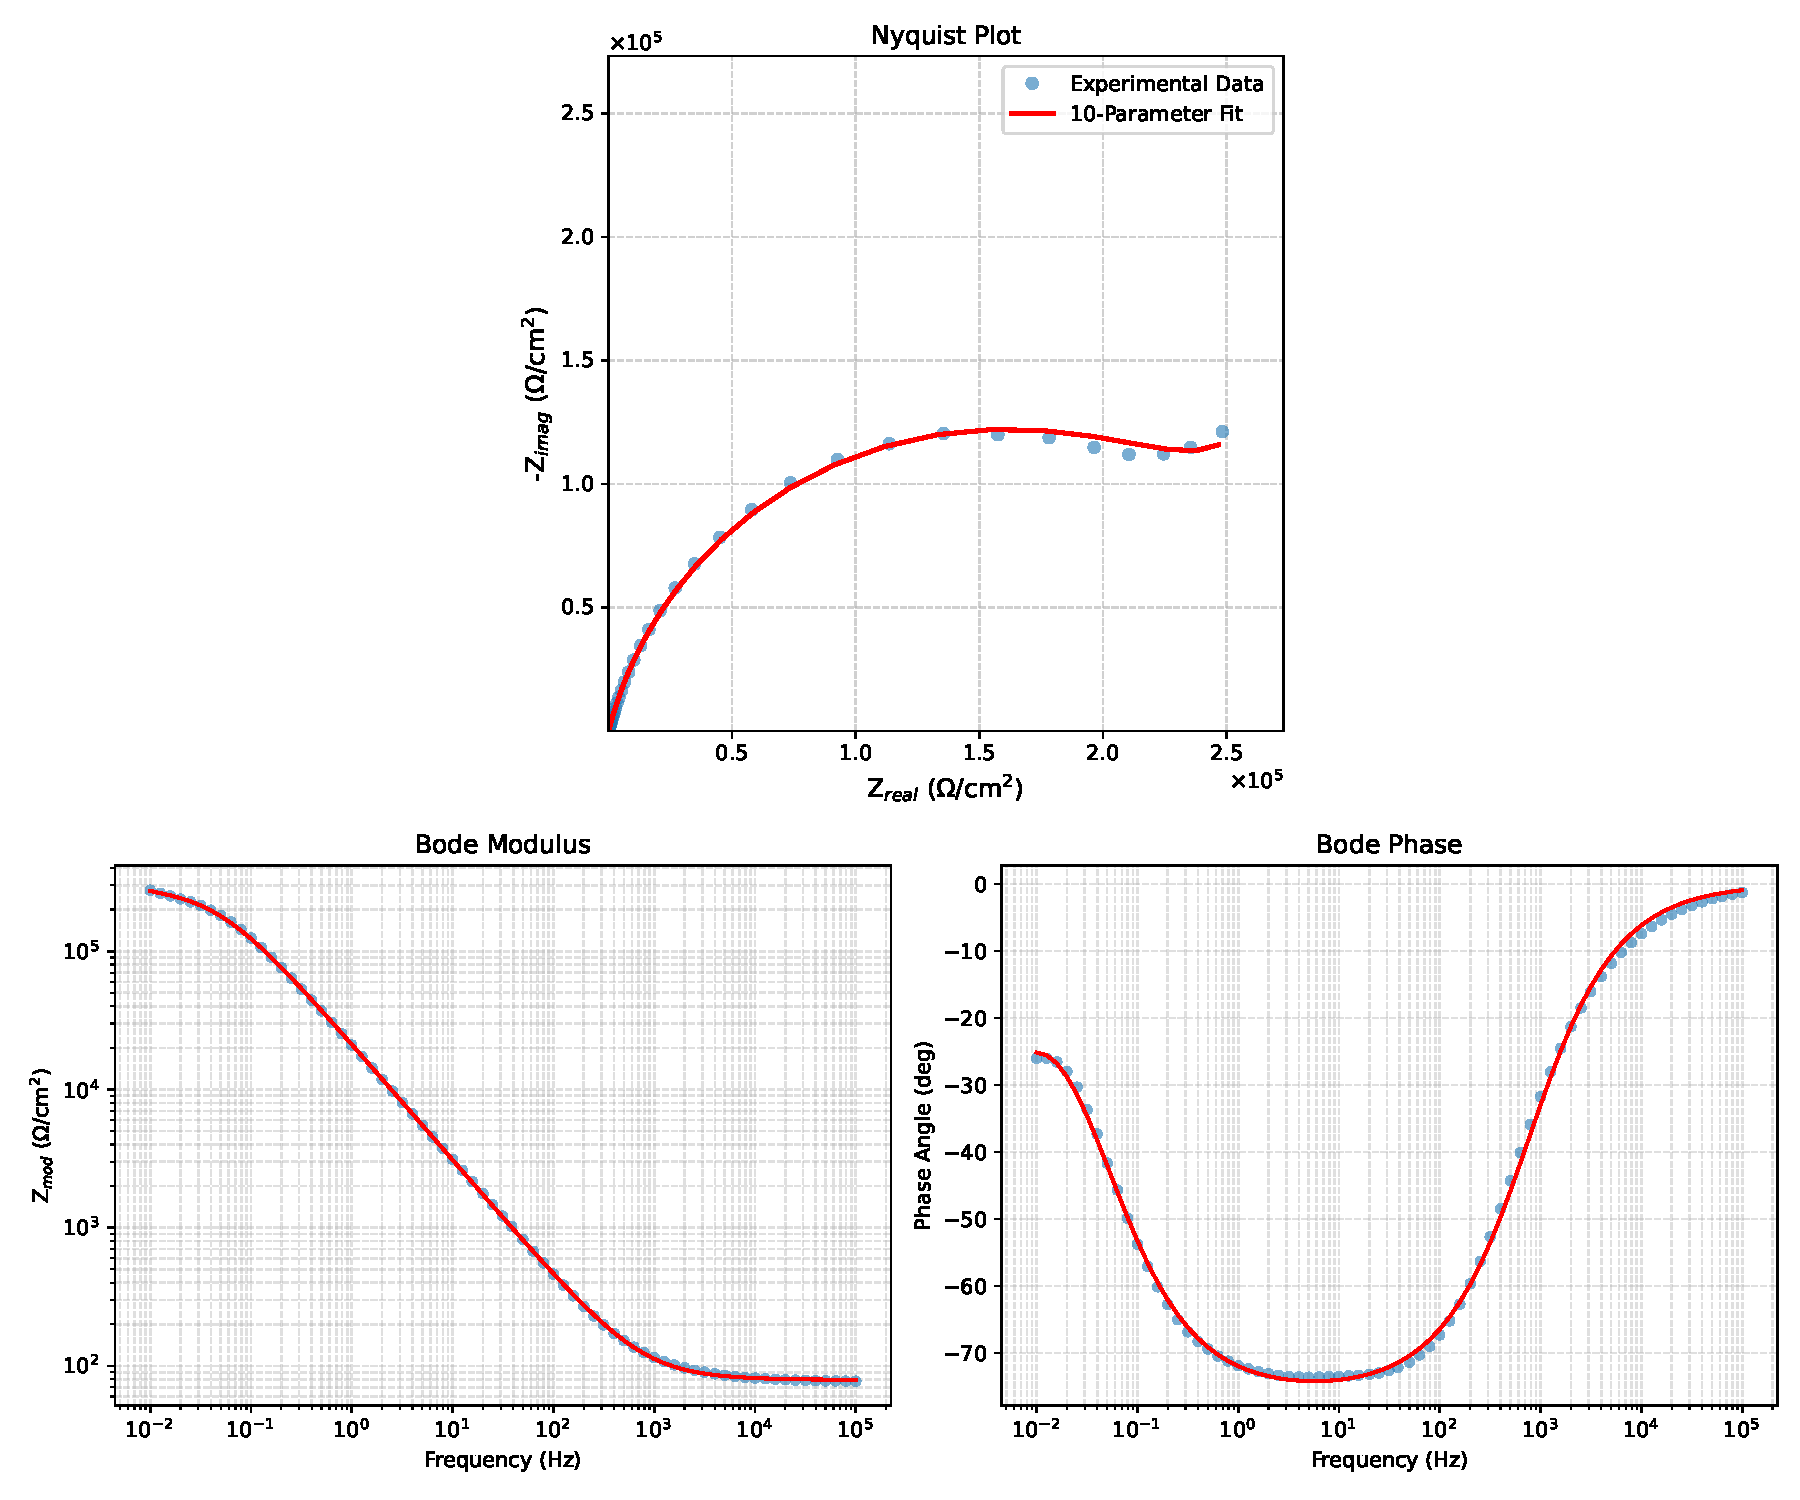
\includegraphics[width=0.7\textwidth]{plots_Cauvel_1_Lcystine_72H.pdf}
    \captionof{figure}{EIS Fit Results for Cauvel\_1\_Lcystine\_72H}
\end{center}

\newpage
\section*{Analysis Results: 168H}
\begin{center}
    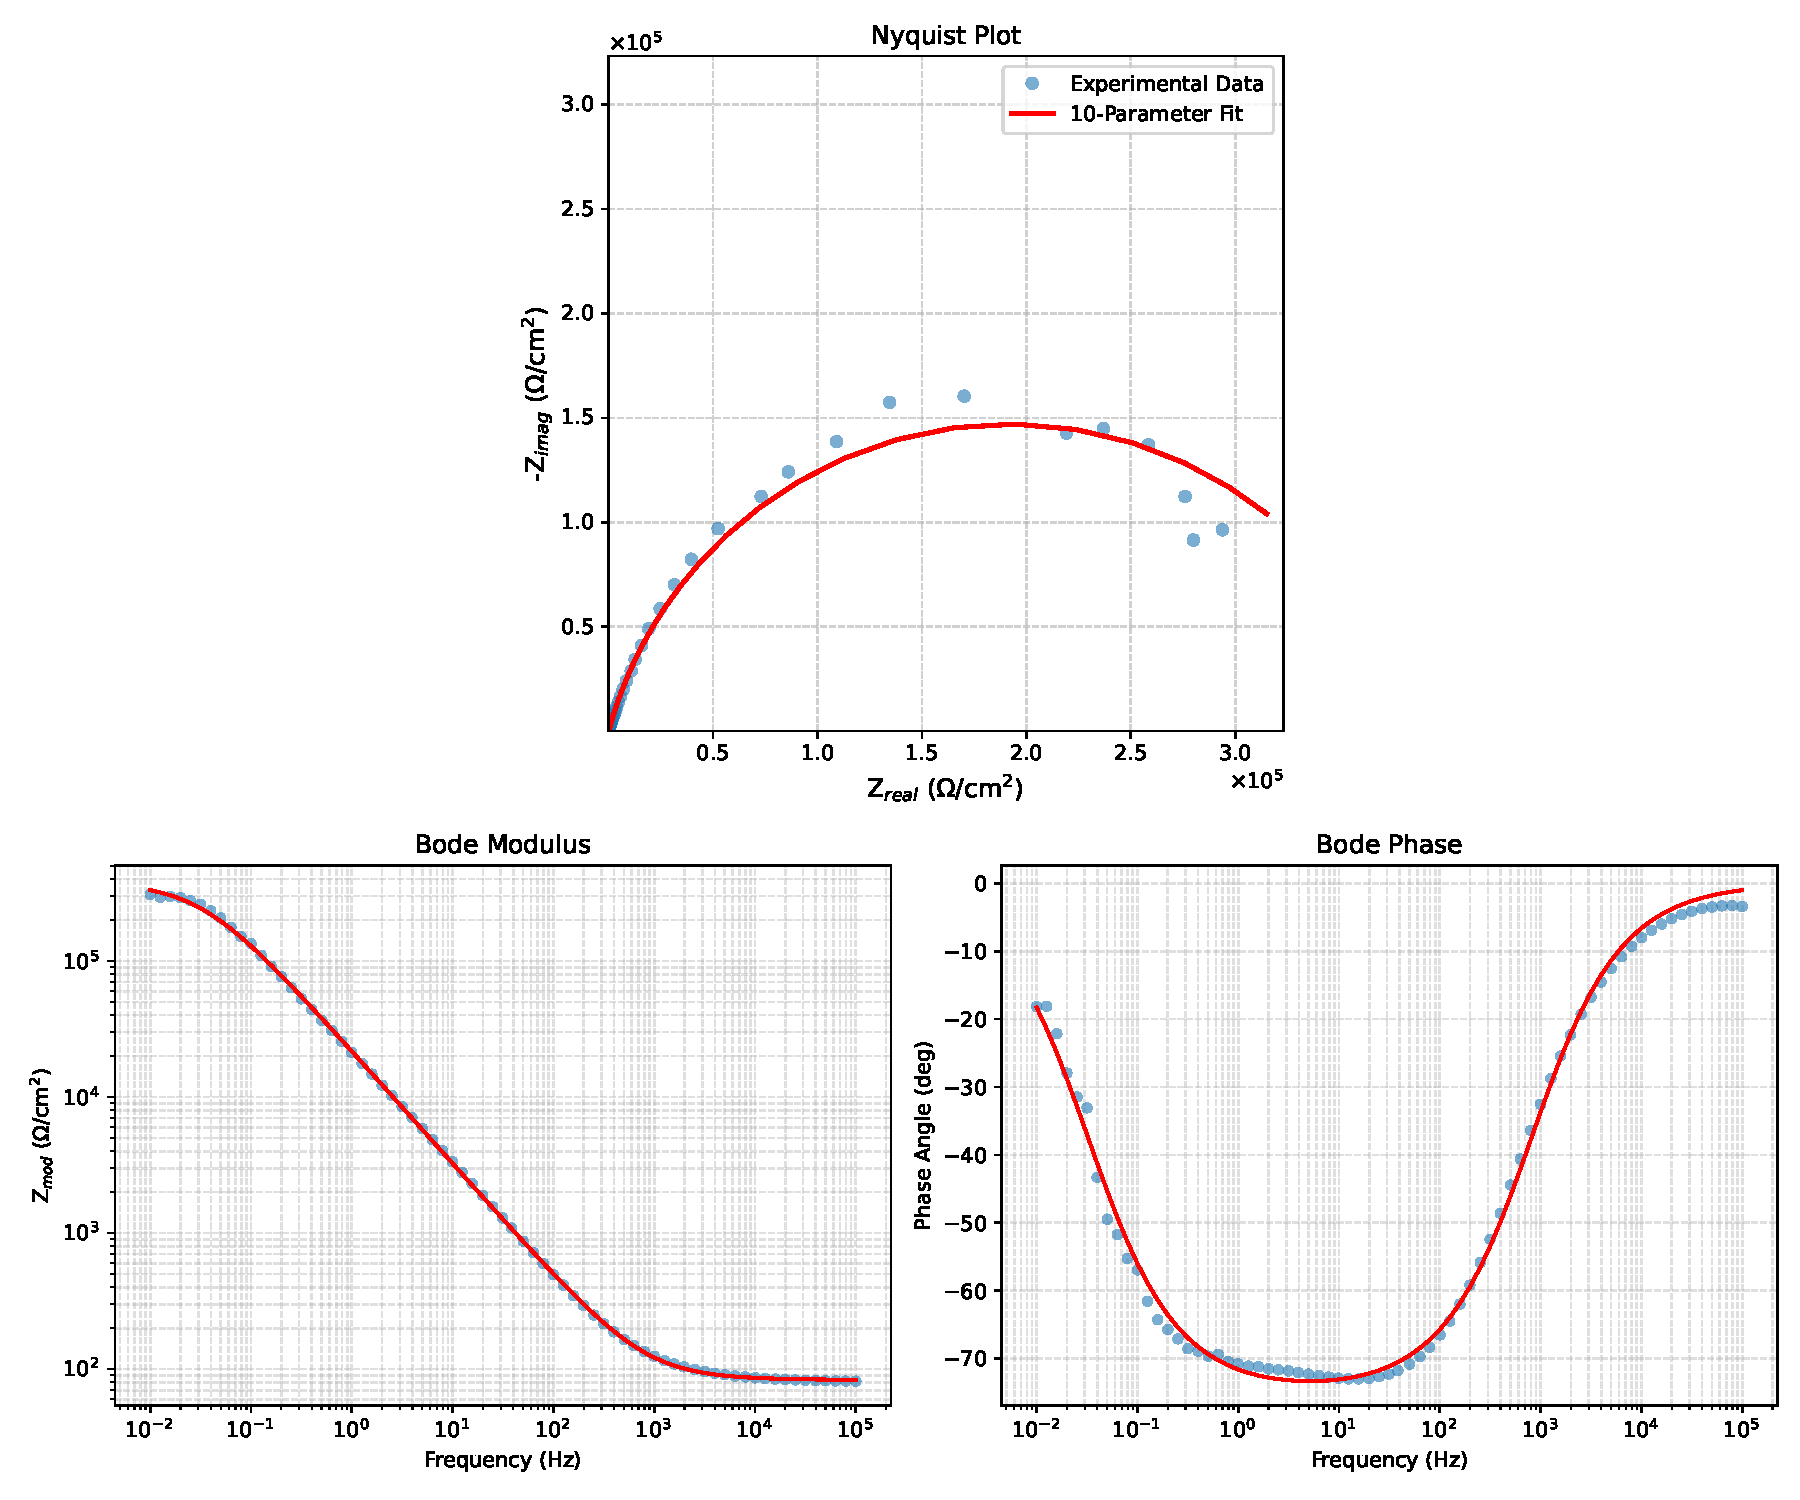
\includegraphics[width=0.7\textwidth]{plots_Cauvel_1_Lcystine_168H.pdf}
    \captionof{figure}{EIS Fit Results for Cauvel\_1\_Lcystine\_168H}
\end{center}


\end{document}
